\chapter{Konzeption\label{chap4:Viertes-Kapitel}}

Um die prototypische Umsetzung einer Search Engine in MCC umzusetzen, werden im folgenden Kapitel verschiedene technische Umsetzungsmöglichkeiten vorgestellt und miteinander verglichen.

% Wird nur eine Volltextsuche oder eine facettierte Volltextsuche umgesetzt?

Im Rahmen dieser Arbeit wird innerhalb der prototypischen Umsetzung nur eine Volltextsuche umgesetzt. Die Umsetzung einer semantischen Suchfunktionalität bedarf der Verwendung eines semantischen Modells, in welchem die begrifflichen Zusammenhänge und Beziehungen definiert sind. Um solch ein wissenbasiertes Modell aufzubauen, wird eine gewisse Datengrundlage benötigt, welche im Umfang des Prototypen nicht gegeben ist.

% Neben der reinen Verwendung von Search Engines, für die Umsetzung einer Suchfunktionalität, gibt es aus technischer Sicht auch die Möglichkeit eine eigene Implementierung auf Basis der Programmbibliothek \glqq Apache Lucene\grqq{} umzusetzen. Eine weitere Möglichkeit ist die Verwendung von DBMS-internen Volltextsuchen. Folgend wird auf die technischen Umsetzungsmöglichkeiten einer Volltextsuche näher eingegangen.

Für das Erstellen eines Gesamtkonzeptes bedarf es einer Validierung der Komponenten \glqq Search Engine\grqq{} und \glqq Datenpipeline\grqq{}. Hierbei beschriebt die Datenpipeline, in welcher Form eine Datenaktualisierung zwischen den Microservices und einer Search Engine umgesetzt werden kann.

Beim Vergleich und der Gegenüberstellung der unterschiedlichen Search Engines, werden die Search Engines \glqq Apache Solr\grqq{} und \glqq Elasticsearch\grqq{} miteinander verglichen. Beide beruhen auf dem Funktionsumfang der Programmbibliothek \glqq Apache Lucene\grqq{}. Da es aus technischer Sicht auch die Möglichkeit gibt eine eigene Search Engine auf Basis von \glqq Apache Lucene\grqq{} zu implementieren, wird jene Programmbibliothek, vor der eigentlichen Auswahl der Search Engine für den Prototypen, erläutert.

Bezüglich der Datenpipeline für die Datenaktualisierung zwischen den Microservices und der Search Engine, werden verschiedene Umsetzungsmöglichkeiten miteinander verglichen. Zu den Konzepten zählen die \glqq Direkte Aktualisierung\grqq{}, die \glqq Pull-or-Push Aktualisierung\grqq{} und die \glqq Change-Data-Capture Aktualisierung\grqq{}.

Nach Auswahl aller benötigten Komponenten wird zum Schluss dieses Kapitels ein Gesamtkonzept erstellt. Jenes Gesamtkonzept ist zudem die Grundlage für die prototypische Umsetzung in \autoref{chap5:Fuenftes-Kapitel}.

% \section{Technische Umsetzung einer Volltextsuche\label{sec4.1:Unterpunkt-1}}

% Bei der technischen Umsetzung einer Volltextsuche dient ein invertierter Index als Grundlage für eingehende Suchanfragen. Hierfür müssen durch Transformationsschritte (siehe auch \autoref{subsec2.1.2:Unterunterpunkt-2}) die Suchphrasen bei der Suchanfrage und die Informationen bei der Indexierung in einer einheitliche Form gebracht werden. Dabei gilt es die morphologischen Varianzen der menschlichen Sprache zu entfernen.

% \subsection{Apache Lucene\label{subsec4.1.1:Unterunterpunkt-1}}

% Inhalt

% \subsection{Search Engine\label{subsec4.1.2:Unterunterpunkt-2}}

% Inhalt

% \subsection{DBMS-interne Volltextsuche\label{subsec4.1.3:Unterunterpunkt-3}}

% Inhalt

\section{Auswahl einer Search Engine\label{sec4.2:Unterpunkt-2}}

Neben einer eigenen Implementierung einer Suchmaschine auf Basis der Programmbibliothek \glqq Apache Lucene\grqq{}, gibt es auf dem Markt bereits ausgereifte Software-Lösungen, welche für die invertierte Indexierung von Daten vorgesehen sind. Im folgenden soll die Auswahl einer solchen Search Engine erfolgen. Jene Search Engine wird nachfolgend in das Gesamtkonzept des Prototypen einfließen. Betrachtet und miteinander verglichen werden dabei die Search Engines \glqq Apache Solr\grqq{} und \glqq Elasticsearch\grqq{}.

\subsection{Vergleichskriterien\label{subsec4.2.1:Unterunterpunkt-1}}

Um die verschiedenen Softwareprodukte für eine Search Engine untereinander zu vergleichen, werden die folgenden Vergleichskriterien verwendet:

\begin{description}
    \item[Lizenzmodelle:]\hfill \\
    Da die jeweilige Search Engine in der Zukunft auch eine Softwarekomponente für das Softwareprodukt MCC sein soll, ist die Verfügbarkeit von kostenfreien Lizenzen ein Vorteil. Auch Lizenzen mit einer einmaligen Bezahlung können für die Verwendung in MCC genutzt werden. Lediglich Lizenzmodelle mit laufenden Kosten (Preis pro Datenvolumen) sind zu vermeiden, da ansonsten bei der einer Skalierung des Kunden die Kosten für eine Nebenkomponente von MCC zu teuer werden.
    
    \begin{itemize}
        \item \textbf{Welche Lizenzmodelle bietet die Search Engine an?}
    \end{itemize}

    \item[Effizienz:]\hfill \\
    Im Umfeld eines Produktionsleitsystems ist die Effizienz einer jeden Softwarekomponente entscheidend. Bei einer Search Engine geht es dabei um die Geschwindigkeit und Ressourcennutzung während der Phase der Indexierung und während der Bearbeitung der Suchanfragen.

    \begin{itemize}
        \item \textbf{In welcher Geschwindigkeit und mit welcher Ressourcennutzung werden bestimmte Mengen von Datensätzen indexiert und durch Suchanfragen durchsucht?}
    \end{itemize}
    
    \item[Rankingmechanismus:]\hfill \\
    Um dem Benutzer eine möglichst aussagekräftige Trefferauflistung zu übergeben, müssen die Suchtreffer nach ihrer Relevanz hin sortiert werden.

    \begin{itemize}
        \item \textbf{Anhand welcher Metrik bestimmt die Search Engine die Relevanz eines Suchtreffers?}
    \end{itemize}

    \item[Dokumentation:]\hfill \\
    Für die Integrierung und Wartung einer Search Engine in das Softwareprodukt MCC ist eine aussagekräftige und umfangreiche Softwaredokumentation von der Search Engine nötig.

    \begin{itemize}
        \item \textbf{Welchen Umfang besitzt die vorliegende Softwaredokumentation?}
    \end{itemize}

\end{description}

\subsection{Programmbibliothek \glqq Apache Lucene\grqq{}\label{subsec4.1.1:Unterunterpunkt-1}}

Für die technische Umsetzung einer Volltextsuche und die damit einhergehende Erstellung und Verwaltung eines invertierten Indexes, bietet sich die frei verfügbare Programmbibliothek \glqq Apache Lucene\grqq{} an.

Lucene, welches anfänglich Ende der 1990er-Jahre von Doug Cutting programmiert wurde, wird seit 2005 als Top-Level-Projekt von der Apache Software Foundation betreut \cite{StefanLuber.2018}.

% Bei der technischen Umsetzung einer Volltextsuche dient ein invertierter Index als Grundlage für eingehende Suchanfragen. Hierfür müssen durch Transformationsschritte (siehe auch \autoref{subsec2.1.2:Unterunterpunkt-2}) die Suchphrasen bei der Suchanfrage und die Informationen bei der Indexierung in einer einheitliche Form gebracht werden. Dabei gilt es die morphologischen Varianzen der menschlichen Sprache zu entfernen.

\subsection{Apache Solr\label{subsec4.2.2:Unterunterpunkt-2}}

Inhalt

\subsection{Elasticsearch\label{subsec4.2.3:Unterunterpunkt-3}}

Inhalt

% \subsection{Sphinx\label{subsec4.2.4:Unterunterpunkt-4}}

% Inhalt

\subsection{Auswahl\label{subsec4.2.5:Unterunterpunkt-5}}

Inhalt

\section{Auswahl einer Datenpipeline für die Datenaktualisierung\label{sec4.3:Unterpunkt-3}}

Für die Erstellung eines invertierten Indexes innerhalb der Search Engine, muss diese mit Daten aus den verschiedenen Microservices befüllt werden. Durch die Verwendung einer geeigneten Datenpipeline kann der invertierte Index innerhalb der Search Engine erzeugt und aktuell gehalten werden. Anhand von Vergleichskriterien werden nachfolgend verschiedene Umsetzungsmöglichkeiten für eine Datenpipeline vorgestellt und anschließend miteinander verglichen.

\subsection{Vergleichskriterien\label{subsec4.3.1:Unterunterpunkt-1}}

Um die verschiedenen Umsetzungsmöglichkeiten für eine Datenpipeline zwischen den Microservices und der Search Engine untereinander zu vergleichen, werden die folgenden Vergleichskriterien verwendet:

\begin{description}
    \item[Mehraufwand bei der Entwicklung:]\hfill \\
    Je nach Art und Umfang der eingesetzten Datenpipeline, entsteht für die Entwickler ein Mehraufwand bei der Umsetzung neuer Funktionalitäten beziehungsweise Microservices.
    
    \begin{itemize}
        \item \textbf{In welchem Umfang ist die Programmierung neuer Funktionalitäten und somit Microservices, von der Einführung einer Search Engine mit dazugehöriger Datenpipeline, betroffen?}
    \end{itemize}

    \item[Datenaktualität:]\hfill \\
    Mit dem Begriff \glqq Datenaktualität\grqq{} wird die Aktualität der Search Engine hinsichtlich der indexierten Daten beschrieben. Dabei gibt die Datenpipeline vor, ob die Indexierung der neuen oder bearbeiteten Objekte in nahezu Echtzeit oder zu einem späteren Zeitpunkt erfolgt.

    \begin{itemize}
        \item \textbf{Wie aktuell sind die Daten innerhalb der Search Engine?}
        \item \textbf{In welcher Zeitspanne gelangen die neuen Daten und Information aus den Speicherschichten der Microservices in die Search Engine?}
    \end{itemize}
    
    % \item[Recovery Funktion:]\hfill \\
    % In dem Anwendungsfall, dass die Search Engine während dem Betrieb neu aufgesetzt werden muss, muss der Aufbau der Datenpipeline eine Recovery Funktion ermöglichen. Unter Recovery Funktion ist dabei die Vollindexierung aller beteiligten Microservices gemeint, wodurch ein invertierter Index in der Search Engine ermöglicht werden kann.
    
    % \begin{itemize}
    %     \item \textbf{Bietet die Datenpipeline eine Möglichkeit der Vollindexierung?}
    % \end{itemize}
    
    \item[Kompatibilität mit Datenbanksystemen:]\hfill \\
    Die eigentlichen Daten und Informationen, welche durch eine Search Engine \glqq durchsuchbar\grqq{} gemacht werden sollen, sind zunächst in den Speicherschichten der jeweiligen Microservices abgespeichert. Durch geeignete Schnittstellenabstraktionen können hierbei unterschiedliche \gls{dbms} für die dauerhafte Speicherung der Daten verwendet werden.

    \begin{itemize}
        \item \textbf{Mit welchen \gls{dbms} ist die jeweilige Datenpipeline kompatibel?}
        \item \textbf{Mit welchem Mehraufwand ist das Verwenden von \glqq neuen\grqq{} \gls{dbms} verbunden?}
    \end{itemize}
    
    \item[Stabilität bei Ausfall von Komponenten:]\hfill \\
    Eine Vermeidung von Komponentenausfällen ist auch in einer Produktionsumgebung nicht zu vermeiden. Die Gründe für den Ausfall einzelner Komponenten können sowohl Hardware-seitig als auch Software-seitig entstehen. Auch Komponenten der Datenpipeline können demnach ausfallen und für einen begrenzten Zeitraum nicht zur Verfügung stehen.

    \begin{itemize}
        \item \textbf{Aus wie vielen Komponenten besteht die Datenpipeline und wie anfällig sind diese für einen Ausfall?}
        \item \textbf{Kann die Datenkonsistenz bei Ausfall einzelner Komponenten der Datenpipeline garantiert werden?}
    \end{itemize}
    
    \item[Auslastung des Systems:]\hfill \\
    Neben der reinen Speicherung der Vorgänge in den Speicherschichten der Microservices muss nun auch die Search Engine mit Daten versorgt werden. Hierfür ist es notwendig Nachrichten zwischen den einzelnen Komponenten auszutauschen. Dieser zusätzliche Nachrichtenaustausch stellt eine zusätzliche Belastung für das System dar und erhöht dessen Auslastung.

    \begin{itemize}
        \item \textbf{In welchem Umfang stellt die Integrierung der Datenpipeline eine zusätzliche Belastung für das System dar?}
    \end{itemize}

    \item[Kompatibilität mit Softwarekomponenten von MCC:]\hfill \\
    Für die spätere Integrierung der Search Engine und der Datenpipeline in das Softwareprodukt MCC ist eine Kompatibilität mit bereits verwendeten Softwarekomponenten von Vorteil. Darunter zählt zum Beispiel der Message Broker \glqq Apache Kafka\grqq{}, welcher bei MCC unteranderem für den Nachrichtenaustausch zwischen den Microservices verwendet wird.

    \begin{itemize}
        \item \textbf{Mit welchen Softwarekomponenten ist die Datenpipeline kompatibel?}
    \end{itemize}

\end{description}

\subsection{Direkte Aktualisierung\label{subsec4.3.2:Unterunterpunkt-2}}

Eine Umsetzungsmöglichkeit für die Datenpipeline ist die direkte Aktualisierung. Führt der Benutzer eine Aktion aus, welche zu einer Änderung der Datenhaltung eines Microservices führt, wird parallel auch ein Search Service über die Aktion informiert. Aktionen, welche mit den Datenhaltungsschichten interagieren, werden auch CRUD-Befehle genannt. CRUD steht dabei für die Aktionen \glqq Create\grqq{}, \glqq Read\grqq{}, \glqq Update\grqq{} und \glqq Delete\grqq{}.

Eine Darstellung der direkten Aktualisierung ist in \autoref{fig:direkte_aktualisierung} abgebildet. Über ein User Interface hat der Benutzer die Möglichkeit mit den Funktionalitäten der Software zu interagieren. Sobald der Benutzer eine Aktion ausführt, welche zu einem CRUD-Befehl führt, wird sowohl der jeweilige Service als auch der Search Service benachrichtigt \footnote{In der \autoref{fig:direkte_aktualisierung} durch eine \glqq 1\grqq{} markiert}. Zu einem späteren Zeitpunkt kann der Benutzer dann über die Suchfunktionalität direkt mit dem Search Service interagieren\footnote{In der \autoref{fig:direkte_aktualisierung} durch eine \glqq 2\grqq{} markiert}.

\begin{figure}[H]
    \centering
    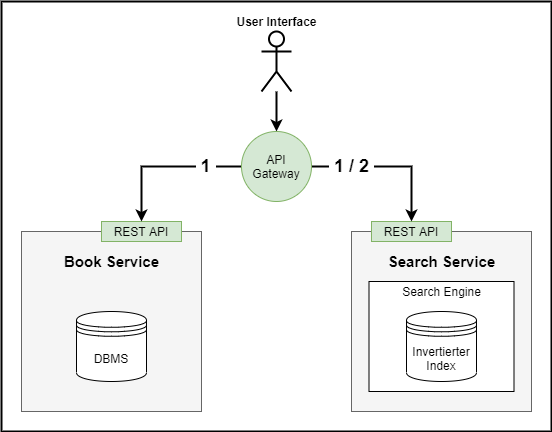
\includegraphics[width=0.6\linewidth]{images/direkte_aktualisierung.png}
    \caption{Datenpipeline: Direkte Aktualisierung}
    \label{fig:direkte_aktualisierung}
\end{figure}

\begin{description}
    \item[Vorteile:]\hfill \\
    Ein Vorteil bei dieser Art der Datenpipeline ist die \textbf{Datenaktualität} innerhalb der Search Engine. Da die CRUD-Befehle nicht nur in die Datenhaltung der Microservice, sondern auch zur Search Engine geschickt werden, findet eine ständige Synchronisation statt.
    
    Für die Datenpipeline werden keine zusätzlichen Softwarekomponenten benötigt und die Kommunikation mit den Datenbanksystemen findet über abstrahierte Schnittstellen der Services statt. Somit sind die Auswahlkriterien bezüglich der \textbf{Kompatibilität mit Datenbanksystemen und Softwarekomponenten von MCC} nicht von Bedeutung, da weder eine direkte Kommunikation mit einem Datenbanksystem, noch eine Verwendung von Softwarekomponenten vorhanden ist.
    
    \item[Nachteile:]\hfill \\
    Die Nachteile einer direkten Aktualisierung liegen beim \textbf{Mehraufwand für die Entwicklung} und Wartung von bestehenden oder neuen Funktionalitäten. Die Entwickler müssen gezielt die einzelnen CRUD-Befehle nicht nur an den eigentlichen Services sondern zusätzlich an den Search Services schicken.

    Ein weiteres Problem ist die \textbf{Datenkonsistenz zwischen Datenhaltung der Microservices und der Search Engine}, sobald eine Komponente des Systems ausfällt. Durch das parallele Benachrichtigen der Microservices und der Search Engine ist die Atomarität der Transaktionen nicht mehr gegeben.

    Bezüglich der \textbf{Auslastung des Systems} besteht bei dieser Art der Datenpipeline das Problem, dass bei jeder Aktion, welche einen CRUD-Befehl beinhaltet ein Nachrichtenaustausch mit dem Search Service stattfindet. Dadurch entsteht eine Engstelle in der Software, durch welche die Performance des gesamten Systems verlangsamt wird.

\end{description}

\subsection{Pull-or-Push Aktualisierung\label{subsec4.3.3:Unterunterpunkt-3}}

Eine weitere Umsetzungsmöglichkeit für die Datenpipeline ist die \glqq Pull-or-Push\grqq{} - Aktualisierung. Hier wird vom Benutzer lediglich die Aktualisierung der eigentlichen Datenhaltung initiiert. Innerhalb einer vordefinierten Zeitspanne werden dann die bearbeiteten Daten entweder mit einem Pull- oder Push-Mechanismus an den Search Service geschickt.

\begin{description}
    \item[Pull:]\hfill \\
    Der Search Service initiiert die Aktualisierung des invertierten Index nach einer vordefinierten Zeitspanne und holt sich dann die Datenänderungen aus den verschiedenen Microservices.
    
    \item[Push:]\hfill \\
    Nach einer vordefinierten Zeitspanne schicken die verschiedenen Microservices die Datenänderungen an den Search Engine, wo dann eine Aktualisierung des invertierten Index stattfinden kann.

\end{description}

In \autoref{fig:pullpush_aktualisierung} ist eine Darstellung der Pull-or-Push Aktualisierung abgebildet. Über das User Interface kann der Benutzer Aktionen initiieren, welche dann von den jeweiligen Microservices bearbeitet werden. Im Falle von CRUD-Befehlen werden lediglich die Datenhaltungsschichten der Microservices benötigt \footnote{In der \autoref{fig:pullpush_aktualisierung} durch eine \glqq 1\grqq{} markiert}. Die Aktualisierung des invertierten Indexes der Search Engine wird zu einem späteren Zeitpunk durch einen Pull- oder Push-Mechanismus durchgeführt \footnote{In der \autoref{fig:pullpush_aktualisierung} durch eine \glqq 2\grqq{} markiert}. Für das stellen einer Suchanfrage kann anschließend der Benutzer direkt mit dem Search Service interagieren \footnote{In der \autoref{fig:pullpush_aktualisierung} durch eine \glqq 3\grqq{} markiert}.

\begin{figure}[H]
    \centering
    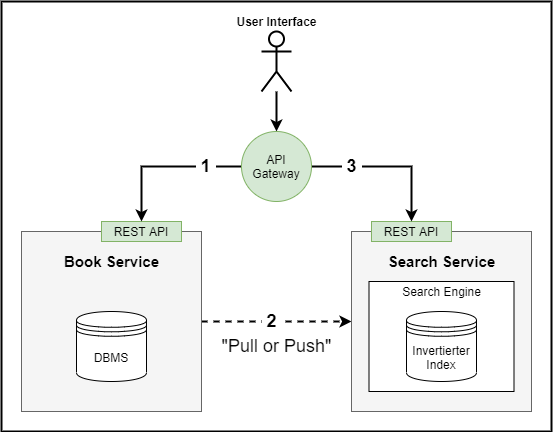
\includegraphics[width=0.6\linewidth]{images/pullpush_aktualisierung.png}
    \caption{Datenpipeline: Pull-or-Push Aktualisierung}
    \label{fig:pullpush_aktualisierung}
\end{figure}

\begin{description}
    \item[Vorteile:]\hfill \\
    Im Gegensatz zur direkten Aktualisierung gibt es bei der Pull-or-Push Aktualisierung keine Engstelle in der Software, da bei jeder Benutzeraktion lediglich die Datenhaltungen der Microservices beeinträchtigt werden. So entsteht durch diese Art der Datenpipeline nur eine minimale \textbf{Mehrbelastung des Systems}.

    Ein weiterer Vorteil ist die \textbf{Kompatibilität bezüglich den Datenbanksystemen und den Softwarekomponenten von MCC}, da hier über vordefinierte Schnittstellen kommuniziert wird.
    
    \item[Nachteile:]\hfill \\
    Ein großer Nachteil bei dieser Datenpipeline ist die \textbf{Datenaktualität} innerhalb der Search Engine. Die Datenaktualität ist dabei von der Zeitspanne des Pull-or-Push Mechanismus abhängig. So kann es bei der Bearbeitung einer Suchanfrage dazu kommen, dass die Search Engine zu dem Zeitpunkt noch nicht aktualisiert wurde und somit eine unvollständige Trefferliste erzeugt wird.

    Bei der Entwicklung und Wartung von neuen Funktionalitäten müssen die Entwickler bei den Pull-or-Push Mechanismen entscheiden, wann die Datenaktualisierung stattfinden soll. Dies resultiert in einen \textbf{Mehraufwand bei der Entwicklung}, da auch definiert werden muss, welche Teile des Datenkontextes \glqq durchsuchbar\grqq{} gemacht werden sollen.

\end{description}

\subsection{Change-Data-Capture Aktualisierung\label{subsec4.3.4:Unterunterpunkt-4}}

Neben der Umsetzungsmöglichkeit der direkten Aktualisierung und der Pull-or-Push Aktualisierung, gibt es noch die Umsetzungsmöglichkeit mithilfe des \gls{cdc} - Pattern. Bei CDC handelt es sich um ein Software Design Pattern, welches die Datenintegration zwischen einer Datenbank und deren Datenquellen definiert \cite{Datenbankenverstehen.de.2021}.

Durch das Beobachten von Datenänderungen in den Quelldatenbanken, ermöglicht \gls{cdc} ein Bewegen und Verarbeiten der Daten in nahezu Echtzeit \cite{JohnKutay.2021}. Somit können Datenreplikationen mit geringer Latenz erzeugt werden. Für die Umsetzung einer CDC-Datenpipeline gibt es vier gängige Methoden \cite{MarkVandeWiel.2021}:

\begin{description}
    \item[Zeitpunkt der letzten Aktualisierung:]\hfill \\
    Um hierbei die Datenbankänderungen mit CDC zu beobachten, müssen die Datenbanktabellen eine \glqq DATE\_MODIFIED\grqq{}-Spalte enthalten, welche den Zeitpunkt der letzten Änderung des Datensatzes protokolliert. Bei der Datensynchronisierung zwischen einer Zieldatenbank und den Quelldatenbanken filtert man nun mithilfe von CDC bezüglich einer solchen \glqq DATE\_MODIFIED\grqq{}-Spalte und entnimmt die Datenänderungen, welche seit der letzten Datenextraktion geändert wurden.

    Ein Problem bei diesem Vorgehen ist das Beobachten von Löschoperationen. Hierbei werden die Datensätze häufig komplett entfernt und ein Beobachten der Spalte \glqq DATE\_MODIFIED\grqq{} ist nicht mehr möglich.

    Auch muss solch eine Spalte für jede Datenbanktabelle zur Verfügung stehen und aktuell gehalten werden. Durch Datenbank-Trigger können diese Spalten aktuell gehalten werden, was jedoch einen erhöhten Overhead verursacht.

    \item[Tabellenunterschiede:]\hfill \\
    Eine weitere Möglichkeit für die Umsetzung einer CDC-Datenpipeline ist das regelmäßige Vergleichen der Tabellenunterschiede. Hierbei wird der aktuelle Zustand der Daten mit dem vorherigen Zustand verglichen.

    Im Vergleich zur Methode, bei welcher man auf die letzte Aktualisierung einer Zeile achtet, können hierbei auch die Löschoperationen berücksichtigt werden. Ein Nachteil ist der hohe Ressourcenverbrauch, welcher bei der Berechnung der Unterschiede zwischen den Datenbeständen entsteht. Somit kann die Methode der Tabellenunterschiede nicht in Echtzeit durchgeführt werden, da für eine ständige Durchführung zu viele Ressourcen benötigt werden.

    \item[Trigger-basierte CDC:]\hfill \\
    Mit der Verwendung von Datenbank-Triggern können Schattentabellen erzeugt werden, auf welchen dann die CDC-Datenpipeline die Änderungen erfassen kann. Hierbei gibt es die Möglichkeit die kompletten Datensätze in eine Schattentabelle zu speichern oder die Möglichkeit lediglich die Primärschlüssel der Datensätze in Verbindung mit der vorgenommen Art der Datenänderung (Einfügen, Aktualisieren oder Löschen) abzuspeichern.

    Bei der Variante der kompletten Speicherung der Datensätze in eine Schattentabelle, entsteht bei der Erstellung und Aktualisierung der Schattentabelle ein Overhead. Ein geringerer Overhead entsteht bei der Variante, wo lediglich die Primärschlüssel mit der Art der Datenänderung in die Schattentabelle gespeichert werden. Hierbei ist aber ein Join zur Quelltabelle nötig, sobald die Datenänderungen ausgelesen werden sollen.

    Somit senkt eine Trigger-basierte CDC-Datenpipeline den Aufwand für die Extraktion der Änderungen, erhöht aber den Aufwand für die Aufzeichnung der Änderungen in den Schattentabellen.

    \item[Log-basierte CDC:]\hfill \\
    Datenbanksysteme speichern alle Änderungen in einem Transaktionsprotokoll, um somit abgebrochene Transaktionen wieder rückgängig zu machen und um die Persistenz der Datenhaltung bei Ausfall des Datenbanksystems zu bewahren. Die Log-basierte CDC-Datenpipeline liest hierbei die Transaktionsprotokolle der Datenbanksysteme und entnimmt daraus die Datenänderungen.

    Ein Problem bei der Verwendung der Transaktionsprotokolle ist der fehlende Standard bezüglich der Art und Weise, wie Änderungen abgespeichert werden. So sind die Transaktionsprotokolle von verschiedenen Datenbankanbietern nach keinem Standart aufgebaut und unterscheiden sich stark voneinander.

\end{description}

Im Rahmen dieser Arbeit und den Umsetzungsmöglichkeiten einer Datenpipeline wird die Log-basierte CDC-Datenpipeline näher betrachtet. In \autoref{fig:changedatacapture_aktualisierung} ist eine Datenpipeline mit einer CDC-Aktualisierung abgebildet. Wie bereits bei der Pull-or-Push Aktualisierung initiiert der Benutzer über ein User Interface eine Aktion, welche dann vom jeweiligen Microservice bearbeitet wird. Werden dabei die Daten der jeweiligen Datenbank durch CRUD-Befehle bearbeitet, werden jene Änderungen auch in den Datenbank-spezifischen Transaktionsprotokollen festgehalten.

Durch die große Varianz der unterschiedlichen Transaktionsprotokolle ist eine eigene Implementierung solch einer CDC-Software umständlich. Abhilfe schafft das Open Source Framework \glqq Debezium\grqq{}, welche auf dem Log-basierten CDC arbeitet und die Änderungen der Transaktionsprotokolle beobachtet.

\begin{description}
\item[Debezium:]\hfill \\
    Nach Luber \cite{StefanLuber.2021} ist Debezium ein Open Source Framework, welches Änderungen in einer Datenbank erfasst und in Form von Event-Streams anderen Anwendungen zur Verfügung stellt. Debezium baut hierbau auf dem Framework \glqq Apache Kafka Connect\grqq{} auf, welches für die Implementierung von Kafka-Schnittstellen verantwortlich ist. Solche Schnittstellen werden entweder in Form von Quellkonnektoren oder Sink-Konnektoren umgesetzt und sind dafür zuständig Datensätze an Kafka zu schicken (Quellkonnektoren) oder Datensätze aus Kafka-Topics (Sink-Konnektoren) an andere Systeme weiterzuschicken \cite{DebeziumCommunity.2021b}.
    
    Debezium bietet derzeit für folgende Datenbankmanagementsysteme Kafka-Konnektoren an: \cite{DebeziumCommunity.2021}

    \begin{itemize}
        \item MongoDB
        \item MySQL
        \item PostgreSQL
        \item SQL Server
        \item Oracle
        \item Db2
    \end{itemize}

    Eine Vorabversion der Kafka-Konnektoren wird bereits für folgende Datenbankmanagementsysteme angeboten: \cite{DebeziumCommunity.2021}

    \begin{itemize}
        \item Cassandra
        \item Vitess
    \end{itemize}

\end{description}

In \autoref{fig:changedatacapture_aktualisierung} ist die Verwendung von Debezium im Gesamtbild der Datenpipeline abgebildet. Zu erkennen ist, das Debezium auf die Transaktionsprotokolle der unterschiedlichen DBMS zugreift und dessen Änderungen an den Message Broker Apache Kafka weiterleitet. Somit fungiert Debezium als Kafka-Produzent und leitet die Datenänderungen aus den Quelldatenbanken an die entsprechenden Kafka-Topics weiter. Um die Daten aus den Kafka-Topics in die jeweilige Search Engine zu leiten, müssen geeignete Kafka-Sink-Konnektoren verwendet werden.

\begin{figure}[H]
    \centering
    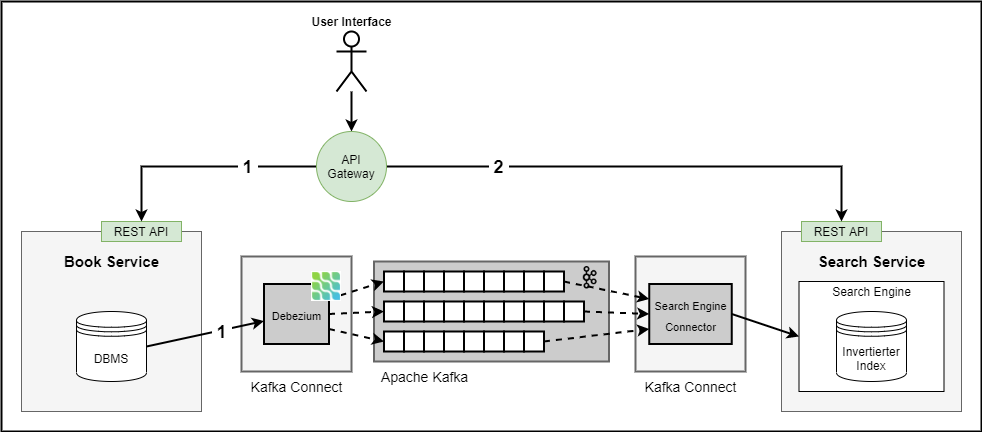
\includegraphics[width=0.9\linewidth]{images/CDC_aktualisierung.png}
    \caption{Datenpipeline: Change-Data-Capture Aktualisierung}
    \label{fig:changedatacapture_aktualisierung}
\end{figure}

\begin{description}
    \item[Vorteile:]\hfill \\
    Ein Vorteil bei der Verwendung der CDC-Aktualisierung liegt bei der \textbf{Echtzeit der Daten} in der jeweiligen Search Engine. Grund dafür ist die stetige Überwachung der DBMS-spezifischen Transaktionsprotokolle.

    In der eigentlichen Software entsteht durch die zusätzliche CDC-Datenpipeline keine Engstelle. Zusätzlich wird durch die stetige Überwachung lediglich ein geringer Datenbestand transportiert, was die \textbf{Auslastung des Gesamtsystems} nicht nachteilig beeinträchtigt.

    Da die verschiedenen Debezium-Kafka-Konnektoren für den Message Broker \glqq Apache Kafka\grqq{} entworfen wurden und jener auch als Basis für den Austausch von Nachrichten in MCC gedacht ist, besteht bei der Verwendung der CDC-Aktualisierung eine hohe \textbf{Kompatibilität mit den Softwarekomponenten} von MCC.
    
    \item[Nachteile:]\hfill \\
    Ein Nachteil ist die Varianz der unterschiedlichen Transaktionsprotokolle. Durch CDC-Software, wie \glqq Debezium\grqq{}, werden die unterschiedlichen Transaktionsprotokolle abstrahiert, jedoch ist man demnach auch von solch einer Software abhängig. So kann Debezium lediglich in Verbindung mit dem Message Broker \glqq Apache Kafka\grqq{} verwendet werden.

\end{description}

\subsection{Auswahl\label{subsec4.3.5:Unterunterpunkt-5}}

Für die Datenpipeline innerhalb der prototypischen Umsetzung wurde sich für die Umsetzungsmöglichkeit \glqq \textbf{Change-Data-Capture Aktualisierung}\grqq{} entschieden. Die Entscheidung resultiert aus einem Vergleich mit den Umsetzungsmöglichkeiten \glqq Direkte Aktualisierung\grqq{} und \glqq Pull-or-Push Aktualisierung\grqq{}.

Eines der wichtigen Vergleichskriterien ist die \textbf{Aktualität der Daten} innerhalb der Search Engine. Die Aktualität jener Daten definiert gleichermaßen die Vollständigkeit von Suchtreffern, welche bei der Search Engine angefragt werden. Da die Datenaktualität bei der Pull-or-Push Aktualisierung abhängig von einer vordefinierten Zeitspanne ist, kann es vorkommen, dass Datenänderungen aufgrund der Zeitspanne noch nicht an die Search Engine übermittelt wurden, aber bei der Search Engine zur gleichen Zeit eine Suchanfrage bezüglich jener Daten erfolgt. Sowohl bei der direkten Aktualisierung, als auch bei der CDC-Aktualisierung werden die Daten zwischen den Microservices und der Search Engine in nahezu Echtzeit aktuell gehalten.

Die verschiedenen Umsetzungsmöglichkeiten unterscheiden sich stark hinsichtlich des \textbf{Mehraufwands für die Entwicklung und Wartung} eines Gesamtsystems. Unter den vorgestellten Umsetzungsmöglichkeiten bietet die CDC-Aktualisierung den geringsten Mehraufwand. Grund hierfür ist die Unabhängigkeit der Datenpipeline bezüglich den internen Implementierungen der einzelnen Microservices, da sich die CDC Aktualisierung ausschließlich direkt mit den entsprechenden Datenhaltungschichten verbindet. Bei Neuentwicklung oder Erweiterungen der Microservices gilt es lediglich die Konfigurationen der CDC-Konnektoren anzupassen, damit bei der CDC Aktualisierung die entsprechenden Datenänderungen in den Datenhaltungsschichten registriert werden. Anders verhält sich der Mehraufwand bei der Umsetzung einer direkten Aktualisierung oder einer Pull-or-Push Aktualisierung. Bei der direkten Aktualisierung liegt die Verantwortung für das Senden der Datenänderungen an den Search Service beim jeweiligen Entwickler. Jener muss neben dem Schreiben der Datenänderungen in die eigentliche Datenhaltung, zusätzlich die Datenänderungen an die Search Engine schicken. Bei Änderungen auf Seiten der Search Engine, gilt es somit alle Funktionalitäten des gesamten Systems zu warten. Bei der Pull-or-Push Aktualisierung ist der Austausch der Datenänderungen zwischen den Microservices und der Search Engine anhand einer Zeitspanne geregelt. Neben der Zeitspanne gilt es auch die Pull- oder Push-Mechanismen zu definieren.

\section{Gesamtkonzept\label{sec4.4:Unterpunkt-4}}

Inhalt